% Activate the following line by filling in the right side. If for example the name of the root file is Main.tex, write
% "...root = Main.tex" if the chapter file is in the same directory, and "...root = ../Main.tex" if the chapter is in a subdirectory.
 
%!TEX root =  
% Activate the following line by filling in the right side. If for example the name of the root file is Main.tex, write
% "...root = Main.tex" if the chapter file is in the same directory, and "...root = ../Main.tex" if the chapter is in a subdirectory.
 
%!TEX root =  

\chapter{Implementation}\label{impl}

\minitoc

\subsection*{Purpose}
This chapter explains the implementation phase of the project it provides a more detailed description of particular key
details that were not decided on in the design phase. This relates in particular to choices regarding the particular CBR algorithms
(k-Nearest Neighbors) and the similarity measures describing how "equal'' two cases are. It also details the data structures that
are used to represent policies and how comparisons are done on these data structures.

\section{Algorithms}

\subsection{K-Nearest Neighbors}\label{kNN}

\emph{K-Nearest Neighbors} (k-NN) is a \emph{lazy, non-parametric} algorithm for classifying objects based on the classification of the nearest examples in a given feature space. k-NN is one of the simplest machine learning algorithms as it decides the classification based on a majority vote of, that is, an object is classified according to the most common classification of its $k$ nearest neighbors. The most critical component for the success of the k-NN algorithms is the definition of distance. This is discussed in Section~\ref{SimilarityMeasures}. 

For testing purposes, we have implemented a very simple kNN that sorts the example set (knowledge base) by distance from the object to be classified and returns the k nearest objects. This is obviously not an optimal approach being $O(n lg(n))$ where $n$ denotes the size of the knowledge base. This is not problematic for a small scale application such as ours where the knowledge contains less than 200 objects. If the system is to be scaled up, it would require a new kNN implementation, of which there are several available.


\subsection{Learning algorithm}\label{learnAlgos}
The learning algorithm is used to update the weights that are used to calculate the distance between policies. These weights are updated when the user overrides a reccomandation from the system. This way the system learns from the users actions, and the next time the system runs it would return with an answer that reflects the users actions more precisely. As an example, let's say that the P3P policy of website X have a field that says that they have the rights to give away the contact-information of their users. So the system reccomends the user to not accept this policy, but the user overrides the recommendation and accepts the policy. Then the learning algorithm is run, and the field(s) that are connected to contact-information are updated. 

\subsubsection{Implemented learning algorithm}
The implemented learning algorithm is a simple one that for each weight-field goes through every policy in the database. And for every policy it checks whether any of its cases have that weight-field. If a policy have that weight-field a counter is incremeted. Then it returns the number of policies (that is accepted) that have this weight-field, divided by the number of total policies. This is as mentioned, done for every weight-field. In figure \ref{pseudoLearnAlg} we have a simplified pseudocode of the learning algorithm.
 
\begin{figure}[htpb]

\begin{verbatim}

countYes=0
countNo=0
containsWeight = false
For weights in database
  For policies in database
    For cases in policy
      If (case contain weight)
        containsWeight=true
    If (containsWeight=true And policy is accepted)
      countYes++
    Else
      countNo++
    newWeight=countYes/(counYes+countNo)	
\end{verbatim}
\caption{Pseudocode for the implemented learning algorithm.}
\label{pseudoLearnAlg}
\end{figure}


\subsection{Confidence Measure}\label{confidenceMeasure}%%TODO Dimitry
%% maybe to be put in design

\subsection{Distance Measures}\label{SimilarityMeasures}%%TODO 

This section discusses the distance measures implemented for comparing two P3P policies. First, it gives a brief overview over the mathematical theory behind distance measures and looks at some standard distance measures. It then looks at what adaptations need to be made to the standard approaches for them to fit the domain of P3P policies.

\subsubsection{Definition}

Mathematically, a \emph{metric} or \emph{distance function} is a function that defines the \emph{distance} between two objects in a set. That is, it defines a notion of how far apart two objects are. In a purely mathematical sense, a distance function defined over a set $X$, $X\times X\longrightarrow \mathbb{R}$ that is required to obey the conditions of non-negativity, symmetry, sub-additivity (the triangle inequality) and identity of indiscernibles. 

Some examples of commonly used metrics are the Eucldean, Mahalanobis, and the Manhattan distance measures. These along with a few others are defined in the next section. These metrics have all in common that $\mathbb{R}^n\times \mathbb{R}^n\longrightarrow \mathbb{R}$, which in the case of comparing privacy policies and corresponding context information, is problematic as these, in their raw form contain large amounts of textual data. Two remedies could be proposed for this situation:

\begin{enumerate}
\item Provide a function to map privacy objects (P3P policies and context info) to real vectors.
\item Define a new metric that operates directly on privacy objects.
\end{enumerate}

%TODO 
%% NBNBNBNB!!!!
%% Formulae must be inserted!!
%%

\subsubsection{Common Metrics}

\begin{itemize}
\item \emph{Manhattan distance} is function computes the distance that would be travelled to get from one data point to the other if a grid-like path is followed. 
\item \emph{Hamming distance} is defined as number of positions in which a source and target vector disagrees.
\item \emph{Levenshtein distance} is based on Hamming distance but adds also operands as insertion, deletion and substitution. 
\item \emph{Ontology distances} are more based on compute semantic similarity of objects rather than their textual representation. For example distance between apple and orange is less then between apple and house. To calculate this distance you need some sort of logical tool like ontological tree. Where every leaf has a logical ancestor for example ancestor for apple will be fruit.
\end{itemize}
\subsubsection{Customer Advice}

In the paper "Towards a Similarity Metric for Comparing Machine Readable Privacy Policies", some of the problems of defining a similarity metric for privacy policies is discussed. A key topic is how the calculation of similarity between online 3P3 policies can be subdivided in two parts, \emph{local similarity} and \emph{global similarity}. This way, known metrics such as Levenshtein distance  can be applied to local distance. And for global similarity we can calculate a simple or weighted average of local distances, where the second one allows for amplifying the importance of particular attributes.

Another important topic is how system designers can apply domain knowledge to improve distance calculation. For example, for the recipient field identifying who data is shared with, there are certain values revealing that significantly more private information is exposed than others. Having private information retained by the website (recipient = "ours") is in a sense less critical than it being given away to third parties for commercial purposes (recipient = "other) or being public (recipient= "public"). So distance between unrelated or public is less than between ours and unrelated.

\subsection{Implementation}

\subsubsection{Bitmap Representation}
A bitmap (or bitstring) is a way of representing a set of objects. It is a mapping from a set to a vector of fixed length, where each member of the set corresponds to a particular entity in the vector. For example over a language $L=\{a,b,c,d\}$ for a sets $\{a,b,c\}$ a bitmap representation will look like $[1, 1, 1, 0]$ where first integer represents $a$ and last integer represents value $d$. This way it doesn't matter what order the values are arranged and how many values are so set $\{d,b\}$ over same language $L$ will be $[0, 1, 0, 1]$ where first value still representing value $a$, or in this case, absence of the item $a$. Calculating intersections or unions over bitmaps $A$ and $B$ uses bitwise Boolean operators. Union can be easily written as $(A_i \vee B_i)$ where $i$ is the position in the vector, and the intersection $(A_i \wedge B_i)$.

Weighed bitmap is when each of the values is multiplied by its corresponding weight. For the language $L$, consider the weights $w_a=1, w_b=2, w_c=4, w_d=3$. Since the bitmap representation of the set $\{a,b,c\}$ is $[1, 1, 1, 0]$, the weighed bit-map will be $[1*w_a, 1*_b, 1*_c, 0*w_d]=[1, 2, 4, 0]$. For another set $\{d,b\}$, it will be $[0, 2, 0, 3]$.

\subsubsection{Privacy Policy Representation}

This section describes the data structures used to represent policies. On the top level, \texttt{policyObject}s contain P3P policy and context information (URL + time etc.). A P3P policy can have a varying number of \emph{statements}, some of them greatly differ from each other, and others are very similar. The privacy policy of www.ticketmaster.com, as displayed in \emph{Privacy Advisor} is shown in Figure~\ref{p3pPol}. In the TicketMaster example, the data items concerned in the policy are the user's name, birth date, home and business contact information as well as a few "technical items". For every of these data items that being described in a policy, we create a \texttt{Case} object inside the \texttt{policyObject}. So in the TicketMaster example, \texttt{user.name} and \texttt{user.bdate} are cases.

\begin{figure}[htbp]
\begin{center}
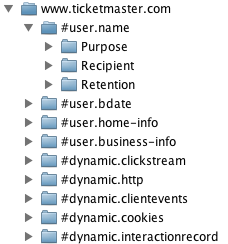
\includegraphics{Implementation/p3p_pol}
\caption{Sample P3P Policy as shown in Privacy Advisor.}
\label{p3pPol}
\end{center}
\end{figure}

Each statement contains of four fields: the type of data collected, purpose, recipient and retention. Purpose, recipient and retention can contain one or many given values, the combination of what describe how the given data-collected may be used in the future. Data-collected is divided in four major fields: dynamic, user, third-party and business. Many different data-types can be collected in one statement. Figure~\ref{p3pNameField} shows TicketMaster's policy with regard to the user's name. In this case we see that TicketMaster stores data for several purposes, both administrative and marketing for an indefinite time period. The statement also reveals that data is shared with unrelated third parties.

\begin{figure}[htbp]
\begin{center}
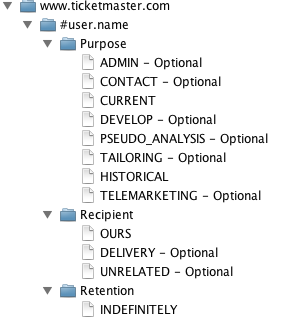
\includegraphics{Implementation/p3p_fields}
\caption{Indepth look at TicketMaster's policy regarding the user's name.}
\label{p3pNameField}
\end{center}
\end{figure}


We then see that a \texttt{Case} contains the purpose, recipient and retention, but a Case can only have one unique data type; this results that one statement can be translated to many cases. \texttt{policyObject} has a list of all its \texttt{Case}s and additional information that we find useful like time of the visit, location of the domain, and action decided upon by the CBR system or the user. Based on SINTEFs proposal the two levels of similarity, local and global are accounted for in implementation. 

\subsubsection{Bitmap Distance}

The distance function is to be a highly modular component of the CBR system. The default distance function implemented uses the bitmap data structure mentioned above, and is henceforth referred to as "Bitmap Distance". For the local similarity Bitmap Distance generates bitmaps for fields, retention, purpose, and recipient. This eliminates the problem that these fields can have a differing number of attributes.  Prior to computing the Hamming distance the bit-map is transformed into weighed bit-map by multiplying every attribute by its weight. Since data-type is a string value the bitmap representation would be impossible. The distance between data-types can be calculated by either string comparison or ontological tree. The Hamming distance for weighed bitmap is easy to implement it can be represented by Boolean expressions. With creation of bitmaps is a fast algorithm with a linear run-time. The easy way of predicting the result and fast run-time is the strengths of this implementation.



\subsubsection{Data-type-string similarity}
The way data type is structured in P3P policies makes it possible to calculate a data-type distance by just parsing data-type-string. Every data-type string has to start with one of the four previously mentioned fields, then after a dot a sub-field is followed after other dot a sub-sub-field. Let us say we have your simplified ontological tree just within the syntax of data-type-string with an "invisible" root node over those four fields. This way when we have two data-type-strings for comparison we can easily count number of ancestors from string A to string B. For instance String A is "user.home-info.postal" and B is "user.bdate". Number of nodes we need to take from stringA to stringB is 3. 

The weakness is that without weights it is more of string comparison than ontological tree.

It is possible to create a weight system so this algorithm will work like a full ontological tree. For example if each node had a value/weight it would be possible to simply take difference between StringA's 1st 2nd and 3rd field and respectfully StringB's fields.
 
Weights are the key to learning and adjusting this algorithm. They are greatly used in previously mentioned implementation of Hamming distance and can give great results in data-type analysis.

\subsubsection{ The global similarity }
The global similarity part was not as easy as creating a bitmap. The number of cases a policy can be is undefined, and the similarity of those cases can differ a great deal. Your solution was sum of minimal distance of each Case to a case in the other policy. For instance a caseA from policyA have distance 2, 3, 1 to cases in policyB that mean the distance caseA will have distance 1 to policyB. 

\begin{figure}[htpb]

\begin{verbatim}

Sum=0
For caseA in PolicyA
  Min=infinity
  For caseB in PolicyB
    Dist=Compare(caseA, caseB)
    If dist<min then
      Min=dist
  Sum=sum+min
Distance=sum
\end{verbatim}

  \caption{Algorithm for similarity computation.}
  \label{similAlgo}
\end{figure}
 

By choosing minimal distance between cases we guaranty that if two cases are identical the distance between them will be 0. But it also creates a problem, consider two policies policyA with {caseA1 caseA2 caseA3} and policyB with {caseB1 caseB2} where every case in A has minimal distance with caseB1. This way the properties of caseB2 will go unnoticed in the sum of distances between cases. We solved this problem by running algorithm twice but changing places of policy A and B the 2nd time and simply summing results.

The weakness of computing this way is that some of the distances will be counted twice, but user-privacy-safety wise is better to count some cases of minimal distance twice then leave a most distant case out.

There is some variations in this method. You can use maximum/minimum distance between cases or average of the sum. We choose minimum because this way we always try to find a best match between cases and policies. With an algorithm that will minimize error from computing twice, from a to b and b to a, minimum distance will give the best results. But in total picture if you use same algorithm that considers every case for every policy in your database the results will be proportional.

\section{Data Storage}

\subsection{Databases}

As the CBR model requires, data must be stored in a persistent fashion between cycles, and thus, while the program is not running. Furthermore, the ability to load raw cases (P3P policies, in this case), is needed not only to initialize a database, especially in a repeatable fashion, but also for establishing the new case under consideration. These requirements are handled by two distinct bodies of code- the P3P parsing class, and the policy database class. Furthermore, there is also the need for a centralized, multi-user database, accessed not locally but across a network, when the local database proves incapable of providing a satisfactory solution to the problem.

\subsection{P3P Parsing}  %Flat File Storage} %% This is what was meant by flat file storage, right??
The \texttt{P3PParser} is used to parse a P3P policy from an XML document to a Java object that can be used by the rest of the framework. The parser is located in the \texttt{parser} group and takes in the path to the xml document as argument. It is based on \texttt{org.xml.sax}, an internal, sequential XML parser in Java.

What it does is sequentially go trough the document, and look at each tag, one by one, dealing only with the tags and attributes we are interested in. It collects information as it parses, and construct a \texttt{PolicyObject} and returns it. The parser also handles custom tags that can be added manually to P3P documents to pre-define action and context for the purpose of bulding a database.

\subsection{Local Database}
The provided local database class (\texttt{PDatabase}) is located in the \texttt{datastorage} group, and implements the abstract model \texttt{PolicyDatabase}. It enforces the singleton model, and is based on \texttt{java.io.serializable} for saving objects on disk, and stores objects in a private \texttt{ArrayList<PolicyObject>}. The methods function precisely as laid out in the Design section, and offer an example of how a PolicyDatabase should function.

Please note the lack of direct access to the internal object storage- thus enabling the use of MySQL, or some other data storage format for not only saving the case history between CBR cycles, but also during the cycle itself, provided that a policy can be added and an iterator provided over the dataset. As with all of the modular classes (algorithms, policy databases, network resources, and user interfaces), the class used to load, interface with, and save the local database can easily be switched out by setting the appropriate  option to the qualified class name in either the configuration file or on command line (in this case, the option is \texttt{policyDB}).

\subsection{Remote Databases}  %network is going here
Access to a community server or network resource is contingent on two things- a remote server, and the class used to interface with said server. In the framework provided, the two classes provide access to a distinct dataset- in fact, while it is possible to create a local substitute providing identical functionality to the existing PolicyDatabase and CBR algorithms, the Java NetworkR class providing the abstract implementation does not provide access to the same case history. Responsibility for providing a reasonable solution in this combined 'retrieve-reuse' phase (the execution of algorithms in a similar model to those used in the local CBR) is intended to reside on the server side, as the resources consumed in transmitting the much larger community case history to a local client are far more significant than those required to run the query locally, and provided only a suggested solution.

Provided in the code is an implementation using a CouchDB database, and a class. The Java code uses several third party libraries (CouchLight and gson, described above) to communicate with a CouchDB database located on a virtual machine provided for the project by NTNU IDI.

\subsubsection{CouchDB server}
The virtual machine hosting the CouchDB server is located at vm-6113.idi.ntnu.no, with the server using port 5984 for communication. All test queries and preliminary code was developed using a set of tools known as \texttt{couchapp} in javascript. The queries can be broken down into two distinct parts: the map-reduce, and the view. 

In CouchDB, a map-reduce operates on a dataset to produce a direct report of the result, with minimal formatting (formatting is possible, but not used in this case). A  map-reduce is composed of a 'map' javascript function, which is applied to every document in the database and can be used to reveal the useful attributes of the document (e.g., the value of an attribute or sum of attributes). This resulting list can be sorted, range-limited, etc. The reduce function is applied to initial results of the associated map function (required), and combines the results in a recursive fashion- the function will be applied to the initial results, then the combined results of the first set of reduce operations, then the second, and so on. 

A view formats the results of a map-reduce operation (offering an easy way to switch between, say, http, xml, and json results, depending on the view applied to a given map-reduce).
The code provided includes a test view that simulates the results of a query- it sends a valid, JSON-encoded Action object that carries the server's suggested solution to the client. A proposal for a map-reduce based on the same algorithms presented above (the k-nearest-neighbors algorithm and conclusion\_simple) is included, but not complete.


\subsubsection{Java Connector Class}
The remote database class provided is entitled \texttt{NRCouchdb}. This class implements the abstract NetworkR class detailed above. The server instance specific options necessary to provide location, port, password, etc, to the class are pulled from the \texttt{NetworkROptions} option, valid at command line as well as in the configuration file. A replacement class should pull any necessary options from a comma-separated list at the same location.

As with all of the modular classes (algorithms, policy databases, network resources, and user interfaces), the fallback resource (usually on a remote server) can easily be switched out by setting the appropriate  option to the qualified class name in either the configuration file or on command line (in this case, the option is \texttt{NetworkRType}).

\section{User Interface} %%TODO 


\subsection{CLI}%%TODO Nicholas




\subsection{GUI}%%TODO Einar

